\documentclass[1p]{elsarticle_modified}
%\bibliographystyle{elsarticle-num}

%\usepackage[colorlinks]{hyperref}
%\usepackage{abbrmath_seonhwa} %\Abb, \Ascr, \Acal ,\Abf, \Afrak
\usepackage{amsfonts}
\usepackage{amssymb}
\usepackage{amsmath}
\usepackage{amsthm}
\usepackage{scalefnt}
\usepackage{amsbsy}
\usepackage{kotex}
\usepackage{caption}
\usepackage{subfig}
\usepackage{color}
\usepackage{graphicx}
\usepackage{xcolor} %% white, black, red, green, blue, cyan, magenta, yellow
\usepackage{float}
\usepackage{setspace}
\usepackage{hyperref}

\usepackage{tikz}
\usetikzlibrary{arrows}

\usepackage{multirow}
\usepackage{array} % fixed length table
\usepackage{hhline}

%%%%%%%%%%%%%%%%%%%%%
\makeatletter
\renewcommand*\env@matrix[1][\arraystretch]{%
	\edef\arraystretch{#1}%
	\hskip -\arraycolsep
	\let\@ifnextchar\new@ifnextchar
	\array{*\c@MaxMatrixCols c}}
\makeatother %https://tex.stackexchange.com/questions/14071/how-can-i-increase-the-line-spacing-in-a-matrix
%%%%%%%%%%%%%%%

\usepackage[normalem]{ulem}

\newcommand{\msout}[1]{\ifmmode\text{\sout{\ensuremath{#1}}}\else\sout{#1}\fi}
%SOURCE: \msout is \stkout macro in https://tex.stackexchange.com/questions/20609/strikeout-in-math-mode

\newcommand{\cancel}[1]{
	\ifmmode
	{\color{red}\msout{#1}}
	\else
	{\color{red}\sout{#1}}
	\fi
}

\newcommand{\add}[1]{
	{\color{blue}\uwave{#1}}
}

\newcommand{\replace}[2]{
	\ifmmode
	{\color{red}\msout{#1}}{\color{blue}\uwave{#2}}
	\else
	{\color{red}\sout{#1}}{\color{blue}\uwave{#2}}
	\fi
}

\newcommand{\Sol}{\mathcal{S}} %segment
\newcommand{\D}{D} %diagram
\newcommand{\A}{\mathcal{A}} %arc


%%%%%%%%%%%%%%%%%%%%%%%%%%%%%5 test

\def\sl{\operatorname{\textup{SL}}(2,\Cbb)}
\def\psl{\operatorname{\textup{PSL}}(2,\Cbb)}
\def\quan{\mkern 1mu \triangleright \mkern 1mu}

\theoremstyle{definition}
\newtheorem{thm}{Theorem}[section]
\newtheorem{prop}[thm]{Proposition}
\newtheorem{lem}[thm]{Lemma}
\newtheorem{ques}[thm]{Question}
\newtheorem{cor}[thm]{Corollary}
\newtheorem{defn}[thm]{Definition}
\newtheorem{exam}[thm]{Example}
\newtheorem{rmk}[thm]{Remark}
\newtheorem{alg}[thm]{Algorithm}

\newcommand{\I}{\sqrt{-1}}
\begin{document}

%\begin{frontmatter}
%
%\title{Boundary parabolic representations of knots up to 8 crossings}
%
%%% Group authors per affiliation:
%\author{Yunhi Cho} 
%\address{Department of Mathematics, University of Seoul, Seoul, Korea}
%\ead{yhcho@uos.ac.kr}
%
%
%\author{Seonhwa Kim} %\fnref{s_kim}}
%\address{Center for Geometry and Physics, Institute for Basic Science, Pohang, 37673, Korea}
%\ead{ryeona17@ibs.re.kr}
%
%\author{Hyuk Kim}
%\address{Department of Mathematical Sciences, Seoul National University, Seoul 08826, Korea}
%\ead{hyukkim@snu.ac.kr}
%
%\author{Seokbeom Yoon}
%\address{Department of Mathematical Sciences, Seoul National University, Seoul, 08826,  Korea}
%\ead{sbyoon15@snu.ac.kr}
%
%\begin{abstract}
%We find all boundary parabolic representation of knots up to 8 crossings.
%
%\end{abstract}
%\begin{keyword}
%    \MSC[2010] 57M25 
%\end{keyword}
%
%\end{frontmatter}

%\linenumbers
%\tableofcontents
%
\newcommand\colored[1]{\textcolor{white}{\rule[-0.35ex]{0.8em}{1.4ex}}\kern-0.8em\color{red} #1}%
%\newcommand\colored[1]{\textcolor{white}{ #1}\kern-2.17ex	\textcolor{white}{ #1}\kern-1.81ex	\textcolor{white}{ #1}\kern-2.15ex\color{red}#1	}

{\Large $\underline{11a_{136}~(K11a_{136})}$}

\setlength{\tabcolsep}{10pt}
\renewcommand{\arraystretch}{1.6}
\vspace{1cm}\begin{tabular}{m{100pt}>{\centering\arraybackslash}m{274pt}}
\multirow{5}{120pt}{
	\centering
	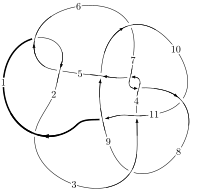
\includegraphics[width=112pt]{../../../GIT/diagram.site/Diagrams/png/385_11a_136.png}\\
\ \ \ A knot diagram\footnotemark}&
\allowdisplaybreaks
\textbf{Linearized knot diagam} \\
\cline{2-2}
 &
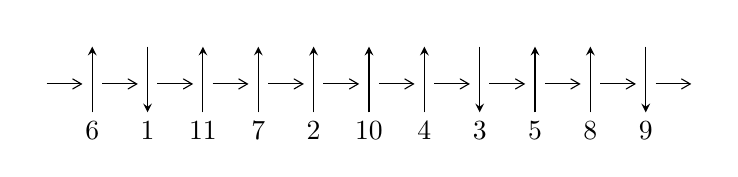
\begin{tikzpicture}[x=20pt, y=17pt]
	% nodes
	\node (C0) at (0, 0) {};
	\node (C1) at (1, 0) {};
	\node (C1U) at (1, +1) {};
	\node (C1D) at (1, -1) {6};

	\node (C2) at (2, 0) {};
	\node (C2U) at (2, +1) {};
	\node (C2D) at (2, -1) {1};

	\node (C3) at (3, 0) {};
	\node (C3U) at (3, +1) {};
	\node (C3D) at (3, -1) {11};

	\node (C4) at (4, 0) {};
	\node (C4U) at (4, +1) {};
	\node (C4D) at (4, -1) {7};

	\node (C5) at (5, 0) {};
	\node (C5U) at (5, +1) {};
	\node (C5D) at (5, -1) {2};

	\node (C6) at (6, 0) {};
	\node (C6U) at (6, +1) {};
	\node (C6D) at (6, -1) {10};

	\node (C7) at (7, 0) {};
	\node (C7U) at (7, +1) {};
	\node (C7D) at (7, -1) {4};

	\node (C8) at (8, 0) {};
	\node (C8U) at (8, +1) {};
	\node (C8D) at (8, -1) {3};

	\node (C9) at (9, 0) {};
	\node (C9U) at (9, +1) {};
	\node (C9D) at (9, -1) {5};

	\node (C10) at (10, 0) {};
	\node (C10U) at (10, +1) {};
	\node (C10D) at (10, -1) {8};

	\node (C11) at (11, 0) {};
	\node (C11U) at (11, +1) {};
	\node (C11D) at (11, -1) {9};
	\node (C12) at (12, 0) {};

	% arrows
	\draw[->,>={angle 60}]
	(C0) edge (C1) (C1) edge (C2) (C2) edge (C3) (C3) edge (C4) (C4) edge (C5) (C5) edge (C6) (C6) edge (C7) (C7) edge (C8) (C8) edge (C9) (C9) edge (C10) (C10) edge (C11) (C11) edge (C12) ;	\draw[->,>=stealth]
	(C1D) edge (C1U) (C2U) edge (C2D) (C3D) edge (C3U) (C4D) edge (C4U) (C5D) edge (C5U) (C6D) edge (C6U) (C7D) edge (C7U) (C8U) edge (C8D) (C9D) edge (C9U) (C10D) edge (C10U) (C11U) edge (C11D) ;
	\end{tikzpicture} \\
\hhline{~~} \\& 
\textbf{Solving Sequence} \\ \cline{2-2} 
 &
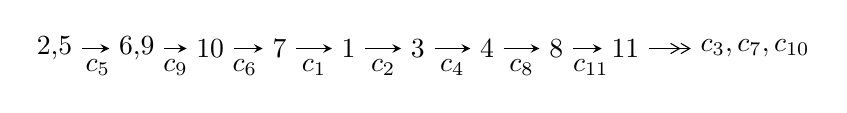
\begin{tikzpicture}[x=25pt, y=7pt]
	% node
	\node (A0) at (-1/8, 0) {2,5};
	\node (A1) at (17/16, 0) {6,9};
	\node (A2) at (17/8, 0) {10};
	\node (A3) at (25/8, 0) {7};
	\node (A4) at (33/8, 0) {1};
	\node (A5) at (41/8, 0) {3};
	\node (A6) at (49/8, 0) {4};
	\node (A7) at (57/8, 0) {8};
	\node (A8) at (65/8, 0) {11};
	\node (C1) at (1/2, -1) {$c_{5}$};
	\node (C2) at (13/8, -1) {$c_{9}$};
	\node (C3) at (21/8, -1) {$c_{6}$};
	\node (C4) at (29/8, -1) {$c_{1}$};
	\node (C5) at (37/8, -1) {$c_{2}$};
	\node (C6) at (45/8, -1) {$c_{4}$};
	\node (C7) at (53/8, -1) {$c_{8}$};
	\node (C8) at (61/8, -1) {$c_{11}$};
	\node (A9) at (10, 0) {$c_{3},c_{7},c_{10}$};

	% edge
	\draw[->,>=stealth]	
	(A0) edge (A1) (A1) edge (A2) (A2) edge (A3) (A3) edge (A4) (A4) edge (A5) (A5) edge (A6) (A6) edge (A7) (A7) edge (A8) ;
	\draw[->>,>={angle 60}]	
	(A8) edge (A9);
\end{tikzpicture} \\ 

\end{tabular} \\

\footnotetext{
The image of knot diagram is generated by the software ``\textbf{Draw programme}" developed by Andrew Bartholomew(\url{http://www.layer8.co.uk/maths/draw/index.htm\#Running-draw}), where we modified some parts for our purpose(\url{https://github.com/CATsTAILs/LinksPainter}).
}\phantom \\ \newline 
\centering \textbf{Ideals for irreducible components\footnotemark of $X_{\text{par}}$} 
 
\begin{align*}
I^u_{1}&=\langle 
-2.54340\times10^{142} u^{97}+2.06865\times10^{143} u^{96}+\cdots+1.58059\times10^{143} b+1.85123\times10^{144},\\
\phantom{I^u_{1}}&\phantom{= \langle  }3.46727\times10^{144} u^{97}-3.34809\times10^{144} u^{96}+\cdots+2.05476\times10^{144} a+2.15518\times10^{145},\\
\phantom{I^u_{1}}&\phantom{= \langle  }u^{98}-2 u^{97}+\cdots-37 u+13\rangle \\
I^u_{2}&=\langle 
u^{16}- u^{15}+4 u^{14}-4 u^{13}+8 u^{12}-8 u^{11}+9 u^{10}-11 u^9+6 u^8-10 u^7+2 u^6-7 u^5-4 u^3+b,\\
\phantom{I^u_{2}}&\phantom{= \langle  }-23 u^{16}+8 u^{15}+\cdots+11 a+8,\\
\phantom{I^u_{2}}&\phantom{= \langle  }u^{17}- u^{16}+4 u^{15}-4 u^{14}+9 u^{13}-9 u^{12}+12 u^{11}-14 u^{10}+11 u^9-15 u^8+6 u^7-13 u^6+2 u^5-8 u^4-3 u^2-1\rangle \\
\\
\end{align*}
\raggedright * 2 irreducible components of $\dim_{\mathbb{C}}=0$, with total 115 representations.\\
\footnotetext{All coefficients of polynomials are rational numbers. But the coefficients are sometimes approximated in decimal forms when there is not enough margin.}
\newpage
\renewcommand{\arraystretch}{1}
\centering \section*{I. $I^u_{1}= \langle -2.54\times10^{142} u^{97}+2.07\times10^{143} u^{96}+\cdots+1.58\times10^{143} b+1.85\times10^{144},\;3.47\times10^{144} u^{97}-3.35\times10^{144} u^{96}+\cdots+2.05\times10^{144} a+2.16\times10^{145},\;u^{98}-2 u^{97}+\cdots-37 u+13 \rangle$}
\flushleft \textbf{(i) Arc colorings}\\
\begin{tabular}{m{7pt} m{180pt} m{7pt} m{180pt} }
\flushright $a_{2}=$&$\begin{pmatrix}0\\u\end{pmatrix}$ \\
\flushright $a_{5}=$&$\begin{pmatrix}1\\0\end{pmatrix}$ \\
\flushright $a_{6}=$&$\begin{pmatrix}1\\- u^2\end{pmatrix}$ \\
\flushright $a_{9}=$&$\begin{pmatrix}-1.68743 u^{97}+1.62943 u^{96}+\cdots-16.4025 u-10.4887\\0.160915 u^{97}-1.30878 u^{96}+\cdots+26.4937 u-11.7123\end{pmatrix}$ \\
\flushright $a_{10}=$&$\begin{pmatrix}-1.52651 u^{97}+0.320645 u^{96}+\cdots+10.0912 u-22.2010\\0.160915 u^{97}-1.30878 u^{96}+\cdots+26.4937 u-11.7123\end{pmatrix}$ \\
\flushright $a_{7}=$&$\begin{pmatrix}2.32231 u^{97}-4.60219 u^{96}+\cdots+99.7785 u-27.3089\\-0.467847 u^{97}+0.927386 u^{96}+\cdots-17.2220 u+8.26210\end{pmatrix}$ \\
\flushright $a_{1}=$&$\begin{pmatrix}- u\\u^3+u\end{pmatrix}$ \\
\flushright $a_{3}=$&$\begin{pmatrix}- u^3\\u^5+u^3+u\end{pmatrix}$ \\
\flushright $a_{4}=$&$\begin{pmatrix}-0.193677 u^{97}+0.576173 u^{96}+\cdots-24.8261 u+19.1249\\0.836899 u^{97}-0.622249 u^{96}+\cdots-0.896403 u+7.44199\end{pmatrix}$ \\
\flushright $a_{8}=$&$\begin{pmatrix}-0.993944 u^{97}-0.792161 u^{96}+\cdots+32.8044 u-33.0338\\0.200388 u^{97}-0.948050 u^{96}+\cdots+20.9776 u-8.91727\end{pmatrix}$ \\
\flushright $a_{11}=$&$\begin{pmatrix}-1.97538 u^{97}+3.67562 u^{96}+\cdots-51.3552 u+15.4260\\0.110979 u^{97}+0.369014 u^{96}+\cdots-8.13883 u+4.87331\end{pmatrix}$\\ \flushright $a_{11}=$&$\begin{pmatrix}-1.97538 u^{97}+3.67562 u^{96}+\cdots-51.3552 u+15.4260\\0.110979 u^{97}+0.369014 u^{96}+\cdots-8.13883 u+4.87331\end{pmatrix}$\\&\end{tabular}
\flushleft \textbf{(ii) Obstruction class $= -1$}\\~\\
\flushleft \textbf{(iii) Cusp Shapes $= -1.93838 u^{97}+4.28511 u^{96}+\cdots-151.895 u+50.7800$}\\~\\
\newpage\renewcommand{\arraystretch}{1}
\flushleft \textbf{(iv) u-Polynomials at the component}\newline \\
\begin{tabular}{m{50pt}|m{274pt}}
Crossings & \hspace{64pt}u-Polynomials at each crossing \\
\hline $$\begin{aligned}c_{1},c_{5}\end{aligned}$$&$\begin{aligned}
&u^{98}-2 u^{97}+\cdots-37 u+13
\end{aligned}$\\
\hline $$\begin{aligned}c_{2}\end{aligned}$$&$\begin{aligned}
&u^{98}+38 u^{97}+\cdots+3909 u+169
\end{aligned}$\\
\hline $$\begin{aligned}c_{3}\end{aligned}$$&$\begin{aligned}
&u^{98}+8 u^{97}+\cdots-2079 u-121
\end{aligned}$\\
\hline $$\begin{aligned}c_{4},c_{7}\end{aligned}$$&$\begin{aligned}
&u^{98}+4 u^{97}+\cdots+23 u+1
\end{aligned}$\\
\hline $$\begin{aligned}c_{6}\end{aligned}$$&$\begin{aligned}
&u^{98}+u^{97}+\cdots-35 u-1
\end{aligned}$\\
\hline $$\begin{aligned}c_{8}\end{aligned}$$&$\begin{aligned}
&u^{98}+u^{97}+\cdots-3372 u+329
\end{aligned}$\\
\hline $$\begin{aligned}c_{9}\end{aligned}$$&$\begin{aligned}
&u^{98}+u^{97}+\cdots-1099 u+29
\end{aligned}$\\
\hline $$\begin{aligned}c_{10}\end{aligned}$$&$\begin{aligned}
&u^{98}-6 u^{97}+\cdots-80 u-3
\end{aligned}$\\
\hline $$\begin{aligned}c_{11}\end{aligned}$$&$\begin{aligned}
&u^{98}+7 u^{97}+\cdots-291 u+55
\end{aligned}$\\
\hline
\end{tabular}\\~\\
\newpage\renewcommand{\arraystretch}{1}
\flushleft \textbf{(v) Riley Polynomials at the component}\newline \\
\begin{tabular}{m{50pt}|m{274pt}}
Crossings & \hspace{64pt}Riley Polynomials at each crossing \\
\hline $$\begin{aligned}c_{1},c_{5}\end{aligned}$$&$\begin{aligned}
&y^{98}+38 y^{97}+\cdots+3909 y+169
\end{aligned}$\\
\hline $$\begin{aligned}c_{2}\end{aligned}$$&$\begin{aligned}
&y^{98}+42 y^{97}+\cdots-1253619 y+28561
\end{aligned}$\\
\hline $$\begin{aligned}c_{3}\end{aligned}$$&$\begin{aligned}
&y^{98}+20 y^{97}+\cdots-1311277 y+14641
\end{aligned}$\\
\hline $$\begin{aligned}c_{4},c_{7}\end{aligned}$$&$\begin{aligned}
&y^{98}+70 y^{97}+\cdots+101 y+1
\end{aligned}$\\
\hline $$\begin{aligned}c_{6}\end{aligned}$$&$\begin{aligned}
&y^{98}+3 y^{97}+\cdots-177 y+1
\end{aligned}$\\
\hline $$\begin{aligned}c_{8}\end{aligned}$$&$\begin{aligned}
&y^{98}+19 y^{97}+\cdots+5038820 y+108241
\end{aligned}$\\
\hline $$\begin{aligned}c_{9}\end{aligned}$$&$\begin{aligned}
&y^{98}+9 y^{97}+\cdots-1350887 y+841
\end{aligned}$\\
\hline $$\begin{aligned}c_{10}\end{aligned}$$&$\begin{aligned}
&y^{98}+10 y^{97}+\cdots-178 y+9
\end{aligned}$\\
\hline $$\begin{aligned}c_{11}\end{aligned}$$&$\begin{aligned}
&y^{98}+3 y^{97}+\cdots-70161 y+3025
\end{aligned}$\\
\hline
\end{tabular}\\~\\
\newpage\flushleft \textbf{(vi) Complex Volumes and Cusp Shapes}
$$\begin{array}{c|c|c}  
\text{Solutions to }I^u_{1}& \I (\text{vol} + \sqrt{-1}CS) & \text{Cusp shape}\\
 \hline 
\begin{aligned}
u &= \phantom{-}0.616891 + 0.784397 I \\
a &= \phantom{-}1.63832 - 0.64003 I \\
b &= -1.090670 + 0.712199 I\end{aligned}
 & -0.34672 - 2.97837 I & \phantom{-0.000000 } 0 \\ \hline\begin{aligned}
u &= \phantom{-}0.616891 - 0.784397 I \\
a &= \phantom{-}1.63832 + 0.64003 I \\
b &= -1.090670 - 0.712199 I\end{aligned}
 & -0.34672 + 2.97837 I & \phantom{-0.000000 } 0 \\ \hline\begin{aligned}
u &= -0.659764 + 0.754623 I \\
a &= -2.07220 - 1.28632 I \\
b &= \phantom{-}1.75363 - 0.61398 I\end{aligned}
 & \phantom{-}0.55151 + 3.39643 I & \phantom{-0.000000 } 0 \\ \hline\begin{aligned}
u &= -0.659764 - 0.754623 I \\
a &= -2.07220 + 1.28632 I \\
b &= \phantom{-}1.75363 + 0.61398 I\end{aligned}
 & \phantom{-}0.55151 - 3.39643 I & \phantom{-0.000000 } 0 \\ \hline\begin{aligned}
u &= -0.496333 + 0.874547 I \\
a &= -0.295450 - 0.901782 I \\
b &= -0.138248 - 1.273140 I\end{aligned}
 & -4.93867 - 2.00874 I & \phantom{-0.000000 } 0 \\ \hline\begin{aligned}
u &= -0.496333 - 0.874547 I \\
a &= -0.295450 + 0.901782 I \\
b &= -0.138248 + 1.273140 I\end{aligned}
 & -4.93867 + 2.00874 I & \phantom{-0.000000 } 0 \\ \hline\begin{aligned}
u &= \phantom{-}0.575791 + 0.810573 I \\
a &= \phantom{-}1.97739 - 0.70589 I \\
b &= -0.88079 - 1.49324 I\end{aligned}
 & \phantom{-}2.03874 + 0.53848 I & \phantom{-0.000000 } 0 \\ \hline\begin{aligned}
u &= \phantom{-}0.575791 - 0.810573 I \\
a &= \phantom{-}1.97739 + 0.70589 I \\
b &= -0.88079 + 1.49324 I\end{aligned}
 & \phantom{-}2.03874 - 0.53848 I & \phantom{-0.000000 } 0 \\ \hline\begin{aligned}
u &= -0.867975 + 0.478153 I \\
a &= -0.836099 - 0.480262 I \\
b &= \phantom{-}0.800077 + 0.888595 I\end{aligned}
 & \phantom{-}1.79924 + 3.99333 I & \phantom{-0.000000 } 0 \\ \hline\begin{aligned}
u &= -0.867975 - 0.478153 I \\
a &= -0.836099 + 0.480262 I \\
b &= \phantom{-}0.800077 - 0.888595 I\end{aligned}
 & \phantom{-}1.79924 - 3.99333 I & \phantom{-0.000000 } 0\\
 \hline 
 \end{array}$$\newpage$$\begin{array}{c|c|c}  
\text{Solutions to }I^u_{1}& \I (\text{vol} + \sqrt{-1}CS) & \text{Cusp shape}\\
 \hline 
\begin{aligned}
u &= \phantom{-}0.632212 + 0.756505 I \\
a &= -1.49685 + 0.04096 I \\
b &= \phantom{-}0.597802 + 0.996584 I\end{aligned}
 & \phantom{-}1.56819 + 1.66106 I & \phantom{-0.000000 } 0 \\ \hline\begin{aligned}
u &= \phantom{-}0.632212 - 0.756505 I \\
a &= -1.49685 - 0.04096 I \\
b &= \phantom{-}0.597802 - 0.996584 I\end{aligned}
 & \phantom{-}1.56819 - 1.66106 I & \phantom{-0.000000 } 0 \\ \hline\begin{aligned}
u &= -0.641246 + 0.799243 I \\
a &= -1.013500 - 0.151324 I \\
b &= \phantom{-}0.905379 + 0.476067 I\end{aligned}
 & \phantom{-}3.77490 - 0.59504 I & \phantom{-0.000000 } 0 \\ \hline\begin{aligned}
u &= -0.641246 - 0.799243 I \\
a &= -1.013500 + 0.151324 I \\
b &= \phantom{-}0.905379 - 0.476067 I\end{aligned}
 & \phantom{-}3.77490 + 0.59504 I & \phantom{-0.000000 } 0 \\ \hline\begin{aligned}
u &= -0.010475 + 1.028500 I \\
a &= \phantom{-}0.405801 - 0.744711 I \\
b &= \phantom{-}0.58430 - 1.48647 I\end{aligned}
 & -7.68730 - 2.02568 I & \phantom{-0.000000 } 0 \\ \hline\begin{aligned}
u &= -0.010475 - 1.028500 I \\
a &= \phantom{-}0.405801 + 0.744711 I \\
b &= \phantom{-}0.58430 + 1.48647 I\end{aligned}
 & -7.68730 + 2.02568 I & \phantom{-0.000000 } 0 \\ \hline\begin{aligned}
u &= -0.440846 + 0.934645 I \\
a &= \phantom{-}1.84346 - 0.35760 I \\
b &= -0.231373 + 0.603261 I\end{aligned}
 & -4.98729 - 2.56981 I & \phantom{-0.000000 } 0 \\ \hline\begin{aligned}
u &= -0.440846 - 0.934645 I \\
a &= \phantom{-}1.84346 + 0.35760 I \\
b &= -0.231373 - 0.603261 I\end{aligned}
 & -4.98729 + 2.56981 I & \phantom{-0.000000 } 0 \\ \hline\begin{aligned}
u &= \phantom{-}0.728651 + 0.628934 I \\
a &= \phantom{-}1.11245 - 1.65306 I \\
b &= -1.25852 + 1.13921 I\end{aligned}
 & -2.36351 - 2.54757 I & \phantom{-0.000000 } 0 \\ \hline\begin{aligned}
u &= \phantom{-}0.728651 - 0.628934 I \\
a &= \phantom{-}1.11245 + 1.65306 I \\
b &= -1.25852 - 1.13921 I\end{aligned}
 & -2.36351 + 2.54757 I & \phantom{-0.000000 } 0\\
 \hline 
 \end{array}$$\newpage$$\begin{array}{c|c|c}  
\text{Solutions to }I^u_{1}& \I (\text{vol} + \sqrt{-1}CS) & \text{Cusp shape}\\
 \hline 
\begin{aligned}
u &= \phantom{-}0.579700 + 0.891928 I \\
a &= -0.246451 + 1.116290 I \\
b &= \phantom{-}1.31896 - 1.31067 I\end{aligned}
 & \phantom{-}1.77426 + 4.06198 I & \phantom{-0.000000 } 0 \\ \hline\begin{aligned}
u &= \phantom{-}0.579700 - 0.891928 I \\
a &= -0.246451 - 1.116290 I \\
b &= \phantom{-}1.31896 + 1.31067 I\end{aligned}
 & \phantom{-}1.77426 - 4.06198 I & \phantom{-0.000000 } 0 \\ \hline\begin{aligned}
u &= -0.103181 + 1.061710 I \\
a &= \phantom{-}0.049091 - 0.616224 I \\
b &= -0.343876 - 0.957178 I\end{aligned}
 & -3.62579 + 0.91604 I & \phantom{-0.000000 } 0 \\ \hline\begin{aligned}
u &= -0.103181 - 1.061710 I \\
a &= \phantom{-}0.049091 + 0.616224 I \\
b &= -0.343876 + 0.957178 I\end{aligned}
 & -3.62579 - 0.91604 I & \phantom{-0.000000 } 0 \\ \hline\begin{aligned}
u &= -1.011860 + 0.341309 I \\
a &= -0.260991 + 0.539760 I \\
b &= \phantom{-}0.436256 - 0.655494 I\end{aligned}
 & -2.16870 - 6.86474 I & \phantom{-0.000000 } 0 \\ \hline\begin{aligned}
u &= -1.011860 - 0.341309 I \\
a &= -0.260991 - 0.539760 I \\
b &= \phantom{-}0.436256 + 0.655494 I\end{aligned}
 & -2.16870 + 6.86474 I & \phantom{-0.000000 } 0 \\ \hline\begin{aligned}
u &= -0.934536 + 0.546067 I \\
a &= \phantom{-}0.851904 + 0.819370 I \\
b &= -0.979519 - 0.722317 I\end{aligned}
 & \phantom{-}4.03924 + 6.33189 I & \phantom{-0.000000 } 0 \\ \hline\begin{aligned}
u &= -0.934536 - 0.546067 I \\
a &= \phantom{-}0.851904 - 0.819370 I \\
b &= -0.979519 + 0.722317 I\end{aligned}
 & \phantom{-}4.03924 - 6.33189 I & \phantom{-0.000000 } 0 \\ \hline\begin{aligned}
u &= \phantom{-}0.929871 + 0.556246 I \\
a &= -0.824388 + 1.097890 I \\
b &= \phantom{-}1.00104 - 1.18467 I\end{aligned}
 & -0.99305 - 12.05120 I & \phantom{-0.000000 } 0 \\ \hline\begin{aligned}
u &= \phantom{-}0.929871 - 0.556246 I \\
a &= -0.824388 - 1.097890 I \\
b &= \phantom{-}1.00104 + 1.18467 I\end{aligned}
 & -0.99305 + 12.05120 I & \phantom{-0.000000 } 0\\
 \hline 
 \end{array}$$\newpage$$\begin{array}{c|c|c}  
\text{Solutions to }I^u_{1}& \I (\text{vol} + \sqrt{-1}CS) & \text{Cusp shape}\\
 \hline 
\begin{aligned}
u &= \phantom{-}0.607517 + 0.904806 I \\
a &= -2.05552 + 1.58210 I \\
b &= \phantom{-}0.895894 + 0.828879 I\end{aligned}
 & -0.72330 + 7.80017 I & \phantom{-0.000000 } 0 \\ \hline\begin{aligned}
u &= \phantom{-}0.607517 - 0.904806 I \\
a &= -2.05552 - 1.58210 I \\
b &= \phantom{-}0.895894 - 0.828879 I\end{aligned}
 & -0.72330 - 7.80017 I & \phantom{-0.000000 } 0 \\ \hline\begin{aligned}
u &= \phantom{-}0.829244 + 0.372367 I \\
a &= -0.920831 + 0.041802 I \\
b &= \phantom{-}0.708117 + 0.178322 I\end{aligned}
 & \phantom{-}1.68869 + 0.41507 I & \phantom{-0.000000 } 0 \\ \hline\begin{aligned}
u &= \phantom{-}0.829244 - 0.372367 I \\
a &= -0.920831 - 0.041802 I \\
b &= \phantom{-}0.708117 - 0.178322 I\end{aligned}
 & \phantom{-}1.68869 - 0.41507 I & \phantom{-0.000000 } 0 \\ \hline\begin{aligned}
u &= -0.637715 + 0.885907 I \\
a &= \phantom{-}1.24620 + 1.12869 I \\
b &= -0.625446 + 0.651293 I\end{aligned}
 & \phantom{-}3.50961 - 4.39996 I & \phantom{-0.000000 } 0 \\ \hline\begin{aligned}
u &= -0.637715 - 0.885907 I \\
a &= \phantom{-}1.24620 - 1.12869 I \\
b &= -0.625446 - 0.651293 I\end{aligned}
 & \phantom{-}3.50961 + 4.39996 I & \phantom{-0.000000 } 0 \\ \hline\begin{aligned}
u &= \phantom{-}0.650522 + 0.909255 I \\
a &= \phantom{-}0.234450 - 0.779015 I \\
b &= -0.934084 + 0.714480 I\end{aligned}
 & \phantom{-}1.10819 + 3.36665 I & \phantom{-0.000000 } 0 \\ \hline\begin{aligned}
u &= \phantom{-}0.650522 - 0.909255 I \\
a &= \phantom{-}0.234450 + 0.779015 I \\
b &= -0.934084 - 0.714480 I\end{aligned}
 & \phantom{-}1.10819 - 3.36665 I & \phantom{-0.000000 } 0 \\ \hline\begin{aligned}
u &= -0.637437 + 0.925557 I \\
a &= \phantom{-}1.30512 + 1.42138 I \\
b &= -2.00689 - 0.34640 I\end{aligned}
 & \phantom{-}0.02639 - 8.44572 I & \phantom{-0.000000 } 0 \\ \hline\begin{aligned}
u &= -0.637437 - 0.925557 I \\
a &= \phantom{-}1.30512 - 1.42138 I \\
b &= -2.00689 + 0.34640 I\end{aligned}
 & \phantom{-}0.02639 + 8.44572 I & \phantom{-0.000000 } 0\\
 \hline 
 \end{array}$$\newpage$$\begin{array}{c|c|c}  
\text{Solutions to }I^u_{1}& \I (\text{vol} + \sqrt{-1}CS) & \text{Cusp shape}\\
 \hline 
\begin{aligned}
u &= \phantom{-}0.961805 + 0.599639 I \\
a &= \phantom{-}0.443570 - 0.416648 I \\
b &= -0.610119 + 0.559112 I\end{aligned}
 & \phantom{-}3.94411 + 0.60196 I & \phantom{-0.000000 } 0 \\ \hline\begin{aligned}
u &= \phantom{-}0.961805 - 0.599639 I \\
a &= \phantom{-}0.443570 + 0.416648 I \\
b &= -0.610119 - 0.559112 I\end{aligned}
 & \phantom{-}3.94411 - 0.60196 I & \phantom{-0.000000 } 0 \\ \hline\begin{aligned}
u &= -0.750684 + 0.850677 I \\
a &= \phantom{-}0.996395 - 0.701894 I \\
b &= \phantom{-}0.18373 + 1.73138 I\end{aligned}
 & \phantom{-}1.41987 - 2.83130 I & \phantom{-0.000000 } 0 \\ \hline\begin{aligned}
u &= -0.750684 - 0.850677 I \\
a &= \phantom{-}0.996395 + 0.701894 I \\
b &= \phantom{-}0.18373 - 1.73138 I\end{aligned}
 & \phantom{-}1.41987 + 2.83130 I & \phantom{-0.000000 } 0 \\ \hline\begin{aligned}
u &= -0.628456 + 0.577625 I \\
a &= -1.49021 - 0.91464 I \\
b &= \phantom{-}0.661533 + 0.370633 I\end{aligned}
 & \phantom{-}0.88936 + 2.15076 I & \phantom{-0.000000 } 0 \\ \hline\begin{aligned}
u &= -0.628456 - 0.577625 I \\
a &= -1.49021 + 0.91464 I \\
b &= \phantom{-}0.661533 - 0.370633 I\end{aligned}
 & \phantom{-}0.88936 - 2.15076 I & \phantom{-0.000000 } 0 \\ \hline\begin{aligned}
u &= -0.147876 + 1.137580 I \\
a &= \phantom{-}0.790358 + 0.086392 I \\
b &= \phantom{-}0.390050 + 1.205370 I\end{aligned}
 & -7.72343 + 2.40963 I & \phantom{-0.000000 } 0 \\ \hline\begin{aligned}
u &= -0.147876 - 1.137580 I \\
a &= \phantom{-}0.790358 - 0.086392 I \\
b &= \phantom{-}0.390050 - 1.205370 I\end{aligned}
 & -7.72343 - 2.40963 I & \phantom{-0.000000 } 0 \\ \hline\begin{aligned}
u &= \phantom{-}0.354450 + 0.773791 I \\
a &= -1.56361 + 0.74448 I \\
b &= \phantom{-}1.330170 + 0.217693 I\end{aligned}
 & \phantom{-}0.304324 - 0.169063 I & \phantom{-0.000000 } 0 \\ \hline\begin{aligned}
u &= \phantom{-}0.354450 - 0.773791 I \\
a &= -1.56361 - 0.74448 I \\
b &= \phantom{-}1.330170 - 0.217693 I\end{aligned}
 & \phantom{-}0.304324 + 0.169063 I & \phantom{-0.000000 } 0\\
 \hline 
 \end{array}$$\newpage$$\begin{array}{c|c|c}  
\text{Solutions to }I^u_{1}& \I (\text{vol} + \sqrt{-1}CS) & \text{Cusp shape}\\
 \hline 
\begin{aligned}
u &= \phantom{-}0.788593 + 0.839284 I \\
a &= \phantom{-}0.246563 + 0.731308 I \\
b &= -0.215213 - 0.162213 I\end{aligned}
 & -0.34003 + 2.94218 I & \phantom{-0.000000 } 0 \\ \hline\begin{aligned}
u &= \phantom{-}0.788593 - 0.839284 I \\
a &= \phantom{-}0.246563 - 0.731308 I \\
b &= -0.215213 + 0.162213 I\end{aligned}
 & -0.34003 - 2.94218 I & \phantom{-0.000000 } 0 \\ \hline\begin{aligned}
u &= \phantom{-}0.254437 + 1.134610 I \\
a &= -0.363254 - 1.220330 I \\
b &= -0.069590 - 0.950170 I\end{aligned}
 & -6.20840 - 0.89525 I & \phantom{-0.000000 } 0 \\ \hline\begin{aligned}
u &= \phantom{-}0.254437 - 1.134610 I \\
a &= -0.363254 + 1.220330 I \\
b &= -0.069590 + 0.950170 I\end{aligned}
 & -6.20840 + 0.89525 I & \phantom{-0.000000 } 0 \\ \hline\begin{aligned}
u &= \phantom{-}0.518432 + 1.055200 I \\
a &= \phantom{-}1.046680 - 0.838479 I \\
b &= -1.019190 - 0.586216 I\end{aligned}
 & -1.13902 + 3.74818 I & \phantom{-0.000000 } 0 \\ \hline\begin{aligned}
u &= \phantom{-}0.518432 - 1.055200 I \\
a &= \phantom{-}1.046680 + 0.838479 I \\
b &= -1.019190 + 0.586216 I\end{aligned}
 & -1.13902 - 3.74818 I & \phantom{-0.000000 } 0 \\ \hline\begin{aligned}
u &= \phantom{-}0.542877 + 1.044420 I \\
a &= -1.82901 + 0.24250 I \\
b &= \phantom{-}0.092857 + 0.401634 I\end{aligned}
 & -4.35388 + 7.97905 I & \phantom{-0.000000 } 0 \\ \hline\begin{aligned}
u &= \phantom{-}0.542877 - 1.044420 I \\
a &= -1.82901 - 0.24250 I \\
b &= \phantom{-}0.092857 - 0.401634 I\end{aligned}
 & -4.35388 - 7.97905 I & \phantom{-0.000000 } 0 \\ \hline\begin{aligned}
u &= -0.622357 + 1.013960 I \\
a &= \phantom{-}1.75460 + 0.58940 I \\
b &= -0.969529 + 0.647486 I\end{aligned}
 & -0.37194 - 7.12003 I & \phantom{-0.000000 } 0 \\ \hline\begin{aligned}
u &= -0.622357 - 1.013960 I \\
a &= \phantom{-}1.75460 - 0.58940 I \\
b &= -0.969529 - 0.647486 I\end{aligned}
 & -0.37194 + 7.12003 I & \phantom{-0.000000 } 0\\
 \hline 
 \end{array}$$\newpage$$\begin{array}{c|c|c}  
\text{Solutions to }I^u_{1}& \I (\text{vol} + \sqrt{-1}CS) & \text{Cusp shape}\\
 \hline 
\begin{aligned}
u &= -0.750313 + 0.925840 I \\
a &= \phantom{-}1.013880 - 0.893072 I \\
b &= -0.101119 + 1.137440 I\end{aligned}
 & -3.57391 - 2.88241 I & \phantom{-0.000000 } 0 \\ \hline\begin{aligned}
u &= -0.750313 - 0.925840 I \\
a &= \phantom{-}1.013880 + 0.893072 I \\
b &= -0.101119 - 1.137440 I\end{aligned}
 & -3.57391 + 2.88241 I & \phantom{-0.000000 } 0 \\ \hline\begin{aligned}
u &= -0.585650 + 1.051210 I \\
a &= -1.77104 - 0.63001 I \\
b &= \phantom{-}1.13257 - 1.51324 I\end{aligned}
 & -4.95576 - 9.43405 I & \phantom{-0.000000 } 0 \\ \hline\begin{aligned}
u &= -0.585650 - 1.051210 I \\
a &= -1.77104 + 0.63001 I \\
b &= \phantom{-}1.13257 + 1.51324 I\end{aligned}
 & -4.95576 + 9.43405 I & \phantom{-0.000000 } 0 \\ \hline\begin{aligned}
u &= \phantom{-}0.665170 + 1.011220 I \\
a &= -2.34754 + 0.55326 I \\
b &= \phantom{-}1.35506 + 1.45199 I\end{aligned}
 & -3.49613 + 7.89288 I & \phantom{-0.000000 } 0 \\ \hline\begin{aligned}
u &= \phantom{-}0.665170 - 1.011220 I \\
a &= -2.34754 - 0.55326 I \\
b &= \phantom{-}1.35506 - 1.45199 I\end{aligned}
 & -3.49613 - 7.89288 I & \phantom{-0.000000 } 0 \\ \hline\begin{aligned}
u &= \phantom{-}0.315902 + 0.719037 I \\
a &= \phantom{-}2.50104 - 1.03660 I \\
b &= \phantom{-}0.448777 - 0.181262 I\end{aligned}
 & -2.69442 - 4.06632 I & -0.58437 + 4.03909 I \\ \hline\begin{aligned}
u &= \phantom{-}0.315902 - 0.719037 I \\
a &= \phantom{-}2.50104 + 1.03660 I \\
b &= \phantom{-}0.448777 + 0.181262 I\end{aligned}
 & -2.69442 + 4.06632 I & -0.58437 - 4.03909 I \\ \hline\begin{aligned}
u &= -0.118535 + 1.224680 I \\
a &= -0.225435 - 0.699797 I \\
b &= -0.369881 - 0.770813 I\end{aligned}
 & -4.06422 + 1.56618 I & \phantom{-0.000000 } 0 \\ \hline\begin{aligned}
u &= -0.118535 - 1.224680 I \\
a &= -0.225435 + 0.699797 I \\
b &= -0.369881 + 0.770813 I\end{aligned}
 & -4.06422 - 1.56618 I & \phantom{-0.000000 } 0\\
 \hline 
 \end{array}$$\newpage$$\begin{array}{c|c|c}  
\text{Solutions to }I^u_{1}& \I (\text{vol} + \sqrt{-1}CS) & \text{Cusp shape}\\
 \hline 
\begin{aligned}
u &= \phantom{-}1.25091\phantom{ +0.000000I} \\
a &= -0.143472\phantom{ +0.000000I} \\
b &= \phantom{-}0.0247908\phantom{ +0.000000I}\end{aligned}
 & \phantom{-}2.39487\phantom{ +0.000000I} & \phantom{-0.000000 } 0 \\ \hline\begin{aligned}
u &= -0.096931 + 1.252370 I \\
a &= -0.095419 + 0.489360 I \\
b &= -0.520535 + 1.177090 I\end{aligned}
 & -8.12216 - 10.14900 I & \phantom{-0.000000 } 0 \\ \hline\begin{aligned}
u &= -0.096931 - 1.252370 I \\
a &= -0.095419 - 0.489360 I \\
b &= -0.520535 - 1.177090 I\end{aligned}
 & -8.12216 + 10.14900 I & \phantom{-0.000000 } 0 \\ \hline\begin{aligned}
u &= \phantom{-}0.123571 + 1.259900 I \\
a &= -0.0030896 + 0.1332200 I \\
b &= \phantom{-}0.228933 + 0.812143 I\end{aligned}
 & -3.19553 + 4.35794 I & \phantom{-0.000000 } 0 \\ \hline\begin{aligned}
u &= \phantom{-}0.123571 - 1.259900 I \\
a &= -0.0030896 - 0.1332200 I \\
b &= \phantom{-}0.228933 - 0.812143 I\end{aligned}
 & -3.19553 - 4.35794 I & \phantom{-0.000000 } 0 \\ \hline\begin{aligned}
u &= -0.622970 + 0.375877 I \\
a &= \phantom{-}0.75207 + 1.49826 I \\
b &= -1.07825 - 1.03683 I\end{aligned}
 & -3.17837 + 4.67663 I & \phantom{-}1.92891 - 3.96631 I \\ \hline\begin{aligned}
u &= -0.622970 - 0.375877 I \\
a &= \phantom{-}0.75207 - 1.49826 I \\
b &= -1.07825 + 1.03683 I\end{aligned}
 & -3.17837 - 4.67663 I & \phantom{-}1.92891 + 3.96631 I \\ \hline\begin{aligned}
u &= -0.664305 + 1.117590 I \\
a &= \phantom{-}1.45034 + 0.74035 I \\
b &= -0.773178 + 1.091240 I\end{aligned}
 & -0.12881 - 9.67930 I & \phantom{-0.000000 } 0 \\ \hline\begin{aligned}
u &= -0.664305 - 1.117590 I \\
a &= \phantom{-}1.45034 - 0.74035 I \\
b &= -0.773178 - 1.091240 I\end{aligned}
 & -0.12881 + 9.67930 I & \phantom{-0.000000 } 0 \\ \hline\begin{aligned}
u &= \phantom{-}0.730610 + 1.090670 I \\
a &= -1.114580 + 0.329073 I \\
b &= \phantom{-}0.657187 + 0.894189 I\end{aligned}
 & \phantom{-}2.40641 + 5.55593 I & \phantom{-0.000000 } 0\\
 \hline 
 \end{array}$$\newpage$$\begin{array}{c|c|c}  
\text{Solutions to }I^u_{1}& \I (\text{vol} + \sqrt{-1}CS) & \text{Cusp shape}\\
 \hline 
\begin{aligned}
u &= \phantom{-}0.730610 - 1.090670 I \\
a &= -1.114580 - 0.329073 I \\
b &= \phantom{-}0.657187 - 0.894189 I\end{aligned}
 & \phantom{-}2.40641 - 5.55593 I & \phantom{-0.000000 } 0 \\ \hline\begin{aligned}
u &= -0.510606 + 1.212630 I \\
a &= -0.717341 - 0.050925 I \\
b &= -0.020678 - 0.617791 I\end{aligned}
 & -5.25124 + 1.21183 I & \phantom{-0.000000 } 0 \\ \hline\begin{aligned}
u &= -0.510606 - 1.212630 I \\
a &= -0.717341 + 0.050925 I \\
b &= -0.020678 + 0.617791 I\end{aligned}
 & -5.25124 - 1.21183 I & \phantom{-0.000000 } 0 \\ \hline\begin{aligned}
u &= \phantom{-}0.709754 + 1.109180 I \\
a &= \phantom{-}1.80382 - 0.46751 I \\
b &= -1.04638 - 1.37372 I\end{aligned}
 & -2.7010 + 18.0711 I & \phantom{-0.000000 } 0 \\ \hline\begin{aligned}
u &= \phantom{-}0.709754 - 1.109180 I \\
a &= \phantom{-}1.80382 + 0.46751 I \\
b &= -1.04638 + 1.37372 I\end{aligned}
 & -2.7010 - 18.0711 I & \phantom{-0.000000 } 0 \\ \hline\begin{aligned}
u &= -0.706931 + 1.111350 I \\
a &= -1.44364 - 0.52370 I \\
b &= \phantom{-}1.07289 - 0.97536 I\end{aligned}
 & \phantom{-}2.29515 - 12.34640 I & \phantom{-0.000000 } 0 \\ \hline\begin{aligned}
u &= -0.706931 - 1.111350 I \\
a &= -1.44364 + 0.52370 I \\
b &= \phantom{-}1.07289 + 0.97536 I\end{aligned}
 & \phantom{-}2.29515 + 12.34640 I & \phantom{-0.000000 } 0 \\ \hline\begin{aligned}
u &= -0.142699 + 0.640237 I \\
a &= \phantom{-}0.34209 + 1.38789 I \\
b &= -1.39818 - 0.54862 I\end{aligned}
 & -2.84596 + 4.76242 I & -1.34751 - 4.70185 I \\ \hline\begin{aligned}
u &= -0.142699 - 0.640237 I \\
a &= \phantom{-}0.34209 - 1.38789 I \\
b &= -1.39818 + 0.54862 I\end{aligned}
 & -2.84596 - 4.76242 I & -1.34751 + 4.70185 I \\ \hline\begin{aligned}
u &= \phantom{-}0.687518 + 1.182220 I \\
a &= \phantom{-}0.704245 - 0.351157 I \\
b &= -0.713048 - 0.294875 I\end{aligned}
 & -0.78309 + 5.33239 I & \phantom{-0.000000 } 0\\
 \hline 
 \end{array}$$\newpage$$\begin{array}{c|c|c}  
\text{Solutions to }I^u_{1}& \I (\text{vol} + \sqrt{-1}CS) & \text{Cusp shape}\\
 \hline 
\begin{aligned}
u &= \phantom{-}0.687518 - 1.182220 I \\
a &= \phantom{-}0.704245 + 0.351157 I \\
b &= -0.713048 + 0.294875 I\end{aligned}
 & -0.78309 - 5.33239 I & \phantom{-0.000000 } 0 \\ \hline\begin{aligned}
u &= \phantom{-}0.561025 + 0.178055 I \\
a &= \phantom{-}1.210090 + 0.465571 I \\
b &= \phantom{-}0.439651 + 0.596445 I\end{aligned}
 & -2.36220 - 3.74881 I & \phantom{-}2.92062 + 2.78211 I \\ \hline\begin{aligned}
u &= \phantom{-}0.561025 - 0.178055 I \\
a &= \phantom{-}1.210090 - 0.465571 I \\
b &= \phantom{-}0.439651 - 0.596445 I\end{aligned}
 & -2.36220 + 3.74881 I & \phantom{-}2.92062 - 2.78211 I \\ \hline\begin{aligned}
u &= -0.477393 + 0.343592 I \\
a &= \phantom{-}0.08519 - 1.52606 I \\
b &= -0.467321 + 0.682390 I\end{aligned}
 & -3.54087 - 1.01143 I & \phantom{-}2.17194 + 3.15617 I \\ \hline\begin{aligned}
u &= -0.477393 - 0.343592 I \\
a &= \phantom{-}0.08519 + 1.52606 I \\
b &= -0.467321 - 0.682390 I\end{aligned}
 & -3.54087 + 1.01143 I & \phantom{-}2.17194 - 3.15617 I \\ \hline\begin{aligned}
u &= \phantom{-}0.462129\phantom{ +0.000000I} \\
a &= -1.40065\phantom{ +0.000000I} \\
b &= \phantom{-}0.814892\phantom{ +0.000000I}\end{aligned}
 & \phantom{-}1.18814\phantom{ +0.000000I} & \phantom{-}6.83070\phantom{ +0.000000I} \\ \hline\begin{aligned}
u &= \phantom{-}0.046008 + 0.429835 I \\
a &= -2.46965 - 1.26206 I \\
b &= -0.053075 + 0.407288 I\end{aligned}
 & \phantom{-}0.60508 + 1.67951 I & \phantom{-}2.80427 - 5.83693 I \\ \hline\begin{aligned}
u &= \phantom{-}0.046008 - 0.429835 I \\
a &= -2.46965 + 1.26206 I \\
b &= -0.053075 - 0.407288 I\end{aligned}
 & \phantom{-}0.60508 - 1.67951 I & \phantom{-}2.80427 + 5.83693 I\\
 \hline 
 \end{array}$$\newpage\newpage\renewcommand{\arraystretch}{1}
\centering \section*{II. $I^u_{2}= \langle u^{16}- u^{15}+\cdots-4 u^3+b,\;-23 u^{16}+8 u^{15}+\cdots+11 a+8,\;u^{17}- u^{16}+\cdots-3 u^2-1 \rangle$}
\flushleft \textbf{(i) Arc colorings}\\
\begin{tabular}{m{7pt} m{180pt} m{7pt} m{180pt} }
\flushright $a_{2}=$&$\begin{pmatrix}0\\u\end{pmatrix}$ \\
\flushright $a_{5}=$&$\begin{pmatrix}1\\0\end{pmatrix}$ \\
\flushright $a_{6}=$&$\begin{pmatrix}1\\- u^2\end{pmatrix}$ \\
\flushright $a_{9}=$&$\begin{pmatrix}2.09091 u^{16}-0.727273 u^{15}+\cdots-2.18182 u-0.727273\\- u^{16}+u^{15}+\cdots+7 u^5+4 u^3\end{pmatrix}$ \\
\flushright $a_{10}=$&$\begin{pmatrix}1.09091 u^{16}+0.272727 u^{15}+\cdots-2.18182 u-0.727273\\- u^{16}+u^{15}+\cdots+7 u^5+4 u^3\end{pmatrix}$ \\
\flushright $a_{7}=$&$\begin{pmatrix}-1.18182 u^{16}+2.45455 u^{15}+\cdots+1.36364 u-1.54545\\0.0909091 u^{16}-0.727273 u^{15}+\cdots+0.818182 u-1.72727\end{pmatrix}$ \\
\flushright $a_{1}=$&$\begin{pmatrix}- u\\u^3+u\end{pmatrix}$ \\
\flushright $a_{3}=$&$\begin{pmatrix}- u^3\\u^5+u^3+u\end{pmatrix}$ \\
\flushright $a_{4}=$&$\begin{pmatrix}-0.272727 u^{16}+0.181818 u^{15}+\cdots-1.45455 u-0.818182\\0.363636 u^{16}+0.0909091 u^{15}+\cdots-0.727273 u+0.0909091\end{pmatrix}$ \\
\flushright $a_{8}=$&$\begin{pmatrix}1.54545 u^{16}-0.363636 u^{15}+\cdots-2.09091 u-1.36364\\-0.818182 u^{16}+1.54545 u^{15}+\cdots-0.363636 u-0.454545\end{pmatrix}$ \\
\flushright $a_{11}=$&$\begin{pmatrix}u^{16}+u^{15}+\cdots-4 u^2+u\\1.36364 u^{16}-1.90909 u^{15}+\cdots-0.727273 u-0.909091\end{pmatrix}$\\ \flushright $a_{11}=$&$\begin{pmatrix}u^{16}+u^{15}+\cdots-4 u^2+u\\1.36364 u^{16}-1.90909 u^{15}+\cdots-0.727273 u-0.909091\end{pmatrix}$\\&\end{tabular}
\flushleft \textbf{(ii) Obstruction class $= 1$}\\~\\
\flushleft \textbf{(iii) Cusp Shapes $= \frac{78}{11} u^{16}-\frac{63}{11} u^{15}+\cdots+\frac{20}{11} u-\frac{8}{11}$}\\~\\
\newpage\renewcommand{\arraystretch}{1}
\flushleft \textbf{(iv) u-Polynomials at the component}\newline \\
\begin{tabular}{m{50pt}|m{274pt}}
Crossings & \hspace{64pt}u-Polynomials at each crossing \\
\hline $$\begin{aligned}c_{1}\end{aligned}$$&$\begin{aligned}
&u^{17}+u^{16}+\cdots+3 u^2+1
\end{aligned}$\\
\hline $$\begin{aligned}c_{2}\end{aligned}$$&$\begin{aligned}
&u^{17}+7 u^{16}+\cdots-6 u-1
\end{aligned}$\\
\hline $$\begin{aligned}c_{3}\end{aligned}$$&$\begin{aligned}
&u^{17}+u^{16}+\cdots-2 u^2-1
\end{aligned}$\\
\hline $$\begin{aligned}c_{4}\end{aligned}$$&$\begin{aligned}
&u^{17}+u^{16}+\cdots+4 u+1
\end{aligned}$\\
\hline $$\begin{aligned}c_{5}\end{aligned}$$&$\begin{aligned}
&u^{17}- u^{16}+\cdots-3 u^2-1
\end{aligned}$\\
\hline $$\begin{aligned}c_{6}\end{aligned}$$&$\begin{aligned}
&u^{17}-2 u^{16}+\cdots+6 u+1
\end{aligned}$\\
\hline $$\begin{aligned}c_{7}\end{aligned}$$&$\begin{aligned}
&u^{17}- u^{16}+\cdots+4 u-1
\end{aligned}$\\
\hline $$\begin{aligned}c_{8}\end{aligned}$$&$\begin{aligned}
&u^{17}+2 u^{15}+\cdots- u-1
\end{aligned}$\\
\hline $$\begin{aligned}c_{9}\end{aligned}$$&$\begin{aligned}
&u^{17}- u^{15}+\cdots+2 u-1
\end{aligned}$\\
\hline $$\begin{aligned}c_{10}\end{aligned}$$&$\begin{aligned}
&u^{17}-9 u^{16}+\cdots+3 u-1
\end{aligned}$\\
\hline $$\begin{aligned}c_{11}\end{aligned}$$&$\begin{aligned}
&u^{17}+8 u^{16}+\cdots+4 u+1
\end{aligned}$\\
\hline
\end{tabular}\\~\\
\newpage\renewcommand{\arraystretch}{1}
\flushleft \textbf{(v) Riley Polynomials at the component}\newline \\
\begin{tabular}{m{50pt}|m{274pt}}
Crossings & \hspace{64pt}Riley Polynomials at each crossing \\
\hline $$\begin{aligned}c_{1},c_{5}\end{aligned}$$&$\begin{aligned}
&y^{17}+7 y^{16}+\cdots-6 y-1
\end{aligned}$\\
\hline $$\begin{aligned}c_{2}\end{aligned}$$&$\begin{aligned}
&y^{17}+3 y^{16}+\cdots-14 y-1
\end{aligned}$\\
\hline $$\begin{aligned}c_{3}\end{aligned}$$&$\begin{aligned}
&y^{17}+y^{16}+\cdots-4 y-1
\end{aligned}$\\
\hline $$\begin{aligned}c_{4},c_{7}\end{aligned}$$&$\begin{aligned}
&y^{17}+11 y^{16}+\cdots-22 y-1
\end{aligned}$\\
\hline $$\begin{aligned}c_{6}\end{aligned}$$&$\begin{aligned}
&y^{17}+4 y^{16}+\cdots+8 y-1
\end{aligned}$\\
\hline $$\begin{aligned}c_{8}\end{aligned}$$&$\begin{aligned}
&y^{17}+4 y^{16}+\cdots- y-1
\end{aligned}$\\
\hline $$\begin{aligned}c_{9}\end{aligned}$$&$\begin{aligned}
&y^{17}-2 y^{16}+\cdots+18 y-1
\end{aligned}$\\
\hline $$\begin{aligned}c_{10}\end{aligned}$$&$\begin{aligned}
&y^{17}+7 y^{16}+\cdots+5 y-1
\end{aligned}$\\
\hline $$\begin{aligned}c_{11}\end{aligned}$$&$\begin{aligned}
&y^{17}+8 y^{16}+\cdots+8 y-1
\end{aligned}$\\
\hline
\end{tabular}\\~\\
\newpage\flushleft \textbf{(vi) Complex Volumes and Cusp Shapes}
$$\begin{array}{c|c|c}  
\text{Solutions to }I^u_{2}& \I (\text{vol} + \sqrt{-1}CS) & \text{Cusp shape}\\
 \hline 
\begin{aligned}
u &= \phantom{-}0.122734 + 0.924960 I \\
a &= -1.00206 - 1.15728 I \\
b &= \phantom{-}0.062667 - 1.123890 I\end{aligned}
 & -6.20661 + 0.55436 I & -3.35974 - 0.56714 I \\ \hline\begin{aligned}
u &= \phantom{-}0.122734 - 0.924960 I \\
a &= -1.00206 + 1.15728 I \\
b &= \phantom{-}0.062667 + 1.123890 I\end{aligned}
 & -6.20661 - 0.55436 I & -3.35974 + 0.56714 I \\ \hline\begin{aligned}
u &= \phantom{-}0.684492 + 0.841900 I \\
a &= -0.793078 - 0.438836 I \\
b &= -0.249155 + 1.355890 I\end{aligned}
 & \phantom{-}2.91021 + 2.64160 I & \phantom{-}11.92622 - 2.88965 I \\ \hline\begin{aligned}
u &= \phantom{-}0.684492 - 0.841900 I \\
a &= -0.793078 + 0.438836 I \\
b &= -0.249155 - 1.355890 I\end{aligned}
 & \phantom{-}2.91021 - 2.64160 I & \phantom{-}11.92622 + 2.88965 I \\ \hline\begin{aligned}
u &= -0.587589 + 0.691285 I \\
a &= -2.12504 - 1.35796 I \\
b &= \phantom{-}1.33891 + 0.47968 I\end{aligned}
 & -1.19877 + 3.86614 I & \phantom{-}3.92641 - 4.92506 I \\ \hline\begin{aligned}
u &= -0.587589 - 0.691285 I \\
a &= -2.12504 + 1.35796 I \\
b &= \phantom{-}1.33891 - 0.47968 I\end{aligned}
 & -1.19877 - 3.86614 I & \phantom{-}3.92641 + 4.92506 I \\ \hline\begin{aligned}
u &= -0.605689 + 0.998898 I \\
a &= \phantom{-}2.08919 + 1.16507 I \\
b &= -1.25998 + 0.86023 I\end{aligned}
 & -2.19753 - 8.63849 I & \phantom{-}2.18255 + 9.85874 I \\ \hline\begin{aligned}
u &= -0.605689 - 0.998898 I \\
a &= \phantom{-}2.08919 - 1.16507 I \\
b &= -1.25998 - 0.86023 I\end{aligned}
 & -2.19753 + 8.63849 I & \phantom{-}2.18255 - 9.85874 I \\ \hline\begin{aligned}
u &= \phantom{-}1.21767\phantom{ +0.000000I} \\
a &= \phantom{-}0.238878\phantom{ +0.000000I} \\
b &= -0.260121\phantom{ +0.000000I}\end{aligned}
 & \phantom{-}2.45771\phantom{ +0.000000I} & \phantom{-}67.1060\phantom{ +0.000000I} \\ \hline\begin{aligned}
u &= -0.250815 + 1.195170 I \\
a &= -0.273838 - 0.517799 I \\
b &= -0.401742 - 0.682852 I\end{aligned}
 & -4.48302 + 1.95126 I & -1.08122 - 8.77138 I\\
 \hline 
 \end{array}$$\newpage$$\begin{array}{c|c|c}  
\text{Solutions to }I^u_{2}& \I (\text{vol} + \sqrt{-1}CS) & \text{Cusp shape}\\
 \hline 
\begin{aligned}
u &= -0.250815 - 1.195170 I \\
a &= -0.273838 + 0.517799 I \\
b &= -0.401742 + 0.682852 I\end{aligned}
 & -4.48302 - 1.95126 I & -1.08122 + 8.77138 I \\ \hline\begin{aligned}
u &= -0.524315 + 0.513369 I \\
a &= \phantom{-}0.591551 - 0.469285 I \\
b &= \phantom{-}0.802273 - 0.099303 I\end{aligned}
 & -1.62681 - 5.44009 I & \phantom{-}4.90727 + 6.73636 I \\ \hline\begin{aligned}
u &= -0.524315 - 0.513369 I \\
a &= \phantom{-}0.591551 + 0.469285 I \\
b &= \phantom{-}0.802273 + 0.099303 I\end{aligned}
 & -1.62681 + 5.44009 I & \phantom{-}4.90727 - 6.73636 I \\ \hline\begin{aligned}
u &= \phantom{-}0.420659 + 0.598526 I \\
a &= \phantom{-}2.25093 - 0.56285 I \\
b &= -0.963143 - 0.483883 I\end{aligned}
 & \phantom{-}1.070290 - 0.654757 I & \phantom{-}6.91810 + 1.92183 I \\ \hline\begin{aligned}
u &= \phantom{-}0.420659 - 0.598526 I \\
a &= \phantom{-}2.25093 + 0.56285 I \\
b &= -0.963143 + 0.483883 I\end{aligned}
 & \phantom{-}1.070290 + 0.654757 I & \phantom{-}6.91810 - 1.92183 I \\ \hline\begin{aligned}
u &= \phantom{-}0.631690 + 1.122780 I \\
a &= -0.857095 + 0.479455 I \\
b &= \phantom{-}0.800233 + 0.266777 I\end{aligned}
 & -1.01115 + 5.13361 I & -3.97273 - 2.25660 I \\ \hline\begin{aligned}
u &= \phantom{-}0.631690 - 1.122780 I \\
a &= -0.857095 - 0.479455 I \\
b &= \phantom{-}0.800233 - 0.266777 I\end{aligned}
 & -1.01115 - 5.13361 I & -3.97273 + 2.25660 I\\
 \hline 
 \end{array}$$\newpage
\newpage\renewcommand{\arraystretch}{1}
\centering \section*{ III. u-Polynomials}
\begin{tabular}{m{50pt}|m{274pt}}
Crossings & \hspace{64pt}u-Polynomials at each crossing \\
\hline $$\begin{aligned}c_{1}\end{aligned}$$&$\begin{aligned}
&(u^{17}+u^{16}+\cdots+3 u^2+1)(u^{98}-2 u^{97}+\cdots-37 u+13)
\end{aligned}$\\
\hline $$\begin{aligned}c_{2}\end{aligned}$$&$\begin{aligned}
&(u^{17}+7 u^{16}+\cdots-6 u-1)(u^{98}+38 u^{97}+\cdots+3909 u+169)
\end{aligned}$\\
\hline $$\begin{aligned}c_{3}\end{aligned}$$&$\begin{aligned}
&(u^{17}+u^{16}+\cdots-2 u^2-1)(u^{98}+8 u^{97}+\cdots-2079 u-121)
\end{aligned}$\\
\hline $$\begin{aligned}c_{4}\end{aligned}$$&$\begin{aligned}
&(u^{17}+u^{16}+\cdots+4 u+1)(u^{98}+4 u^{97}+\cdots+23 u+1)
\end{aligned}$\\
\hline $$\begin{aligned}c_{5}\end{aligned}$$&$\begin{aligned}
&(u^{17}- u^{16}+\cdots-3 u^2-1)(u^{98}-2 u^{97}+\cdots-37 u+13)
\end{aligned}$\\
\hline $$\begin{aligned}c_{6}\end{aligned}$$&$\begin{aligned}
&(u^{17}-2 u^{16}+\cdots+6 u+1)(u^{98}+u^{97}+\cdots-35 u-1)
\end{aligned}$\\
\hline $$\begin{aligned}c_{7}\end{aligned}$$&$\begin{aligned}
&(u^{17}- u^{16}+\cdots+4 u-1)(u^{98}+4 u^{97}+\cdots+23 u+1)
\end{aligned}$\\
\hline $$\begin{aligned}c_{8}\end{aligned}$$&$\begin{aligned}
&(u^{17}+2 u^{15}+\cdots- u-1)(u^{98}+u^{97}+\cdots-3372 u+329)
\end{aligned}$\\
\hline $$\begin{aligned}c_{9}\end{aligned}$$&$\begin{aligned}
&(u^{17}- u^{15}+\cdots+2 u-1)(u^{98}+u^{97}+\cdots-1099 u+29)
\end{aligned}$\\
\hline $$\begin{aligned}c_{10}\end{aligned}$$&$\begin{aligned}
&(u^{17}-9 u^{16}+\cdots+3 u-1)(u^{98}-6 u^{97}+\cdots-80 u-3)
\end{aligned}$\\
\hline $$\begin{aligned}c_{11}\end{aligned}$$&$\begin{aligned}
&(u^{17}+8 u^{16}+\cdots+4 u+1)(u^{98}+7 u^{97}+\cdots-291 u+55)
\end{aligned}$\\
\hline
\end{tabular}\newpage\renewcommand{\arraystretch}{1}
\centering \section*{ IV. Riley Polynomials}
\begin{tabular}{m{50pt}|m{274pt}}
Crossings & \hspace{64pt}Riley Polynomials at each crossing \\
\hline $$\begin{aligned}c_{1},c_{5}\end{aligned}$$&$\begin{aligned}
&(y^{17}+7 y^{16}+\cdots-6 y-1)(y^{98}+38 y^{97}+\cdots+3909 y+169)
\end{aligned}$\\
\hline $$\begin{aligned}c_{2}\end{aligned}$$&$\begin{aligned}
&(y^{17}+3 y^{16}+\cdots-14 y-1)(y^{98}+42 y^{97}+\cdots-1253619 y+28561)
\end{aligned}$\\
\hline $$\begin{aligned}c_{3}\end{aligned}$$&$\begin{aligned}
&(y^{17}+y^{16}+\cdots-4 y-1)(y^{98}+20 y^{97}+\cdots-1311277 y+14641)
\end{aligned}$\\
\hline $$\begin{aligned}c_{4},c_{7}\end{aligned}$$&$\begin{aligned}
&(y^{17}+11 y^{16}+\cdots-22 y-1)(y^{98}+70 y^{97}+\cdots+101 y+1)
\end{aligned}$\\
\hline $$\begin{aligned}c_{6}\end{aligned}$$&$\begin{aligned}
&(y^{17}+4 y^{16}+\cdots+8 y-1)(y^{98}+3 y^{97}+\cdots-177 y+1)
\end{aligned}$\\
\hline $$\begin{aligned}c_{8}\end{aligned}$$&$\begin{aligned}
&(y^{17}+4 y^{16}+\cdots- y-1)(y^{98}+19 y^{97}+\cdots+5038820 y+108241)
\end{aligned}$\\
\hline $$\begin{aligned}c_{9}\end{aligned}$$&$\begin{aligned}
&(y^{17}-2 y^{16}+\cdots+18 y-1)(y^{98}+9 y^{97}+\cdots-1350887 y+841)
\end{aligned}$\\
\hline $$\begin{aligned}c_{10}\end{aligned}$$&$\begin{aligned}
&(y^{17}+7 y^{16}+\cdots+5 y-1)(y^{98}+10 y^{97}+\cdots-178 y+9)
\end{aligned}$\\
\hline $$\begin{aligned}c_{11}\end{aligned}$$&$\begin{aligned}
&(y^{17}+8 y^{16}+\cdots+8 y-1)(y^{98}+3 y^{97}+\cdots-70161 y+3025)
\end{aligned}$\\
\hline
\end{tabular}
\vskip 2pc
\end{document}